\documentclass[border=8pt]{standalone}
\usepackage{amsmath}
\usepackage{pgfplots}
\pgfplotsset{compat=1.18}
\usepgfplotslibrary{fillbetween}
\begin{document}
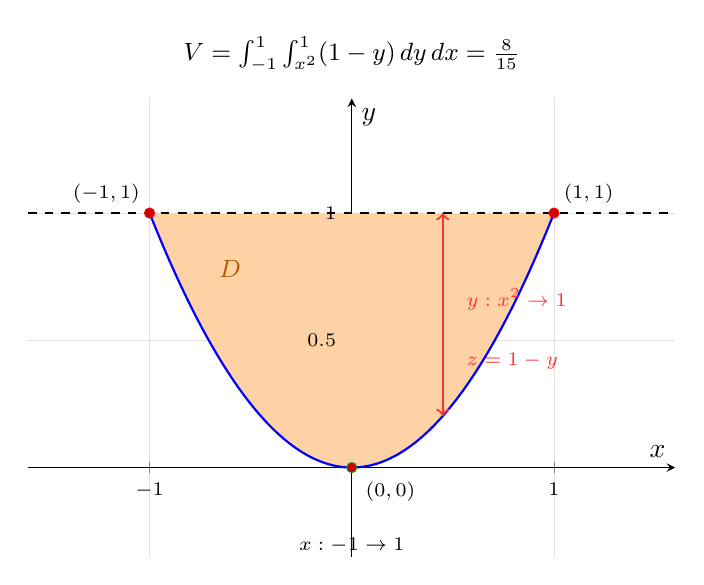
\begin{tikzpicture}
\begin{axis}[
    width=9.8cm, height=7.4cm,
    xlabel={$x$}, ylabel={$y$},
    xmin=-1.6, xmax=1.6, ymin=-0.35, ymax=1.45,
    ytick={0,0.5,1}, xtick={-1,0,1},
    tick label style={font=\scriptsize}, label style={font=\small},
    title style={font=\small},
    axis lines=middle,
    grid=major, grid style={black!12, line width=0.3pt},
    title={$V=\int_{-1}^{1}\int_{x^{2}}^{1}(1-y)\,dy\,dx=\frac{8}{15}$},
    samples=120, domain=-1:1,
]
\addplot+[name path=parab, thick, blue, mark=none, forget plot] {x^2};
\addplot+[name path=top, thick, dashed, black, mark=none, forget plot, domain=-1.6:1.6] {1};
\addplot[orange!35, draw=none] fill between[of=parab and top, soft clip={domain=-1:1}];
% typical vertical strip
\draw[red!80, thick, <->] (axis cs:0.45,0.2025) -- (axis cs:0.45,1);
\node[font=\scriptsize, red!80, anchor=west] at (axis cs:0.52,0.66) {$y:x^{2}\to 1$};
\node[font=\scriptsize, red!80, anchor=west] at (axis cs:0.52,0.42) {$z=1-y$};
% corner points
\addplot+[only marks, mark=*, red, mark size=1.8pt, forget plot] coordinates {(-1,1) (1,1)};
\addplot+[only marks, mark=*, green!60!black, mark size=1.8pt, forget plot] coordinates {(0,0)};
\node[font=\scriptsize, anchor=south east] at (axis cs:-1,1) {$(-1,1)$};
\node[font=\scriptsize, anchor=south west] at (axis cs:1,1) {$(1,1)$};
\node[font=\scriptsize, anchor=north west] at (axis cs:0.02,-0.02) {$(0,0)$};
\node[font=\scriptsize, anchor=north] at (axis cs:0,-0.24) {$x:-1\to 1$};
\node[font=\small, orange!70!black, anchor=east] at (axis cs:-0.5,0.78) {$D$};
\end{axis}
\end{tikzpicture}
\end{document}
